\section{Rules Engines}

\subsection{What Is A Rules Engine?}

In this section, we will describe what a rules engine is and a little of its history.

The Aristotelian doctrine of essentialism declares that a thing has essential properties and properties that are accidental.
If one takes away the accidental properties of a thing, then the thing remains the thing.
In contrast, if one takes away the thing's essential properties, the thing is no longer the thing.
If the ``thing'' we refer to is a business application, its essential properties are its business rules.

Simply put, business rules are the principles or regulations by which an organization carries out the tasks needed to achieve its goals.
When adequately defined, it is possible to encode these rules into statements that define or constrain some business organizational behaviour.
A rule consists of a condition and an action.
When the condition is satisfied, then the action is performed.
More formally, business rules follow the logical principle of Modus Ponens.

When described like this, one could imagine this as just the ``if-then'' logic frequently used in traditional programming.
One would not be wrong. 
However, representing all the combinatorial outcomes of an extensive collection of rules in traditional programming can become complex.
Each additional rule adds to the fragility.
Additionally, developers tend to distribute rules throughout the source code or database of the application.

We find descriptions of these rules in the design documentation or user manuals.
However, as applications evolve, documentation gets out of sync with the codebase.
Once desynchronization occurs, to know the rules governing the application, one has to navigate the codebase and decode the rules from often scattered locations.

A rules engine is also known as a Business Rules Engine, a Business Rules Management System or a Production Rules System.

Rules Engines are declarative, focussing on the what of the rules, not the how of the execution.
Date\cite{date2000not} describes a rules engine role as ``to specify business process declaratively, via business rules and get the system to compile those rules into the necessary procedural (and executable) code.''
Fowler\cite{Fowler_rulesEngine} describes a rules engine as follows: `` ... providing an alternative computational model.
Instead of the usual imperative model, which consists of commands in sequence with conditionals and loops, a rules engine is based on a Production Rule System.
This is a set of production rules, each of which has a condition and an action ...''.

The goal of a rules engine is to abstract business rules into encoded and packaged logic that defines the tasks of an organization with the accompanying tools that evaluate and execute these rules.
Simply put, they are where we evaluate our rules.
Rules engines match rules against facts and infer conclusions.
Returning to the Modus Ponens comparison:

\begin{tabular}{c@{\,}l@{}} 
    & $p$ \\
\arrayrulecolor{blue!60!green!70}    & $p \to q$ \\\cline{2-2}
$\therefore$         & $q$ \\
\end{tabular}

If the premise $p$ holds and the implication $p \to q$ holds, then the conclusion $q$ holds.
In terms of a rule engine and business rules, this would be:
\begin{enumerate}
    \setlength\itemsep{0em}
    \item the rules engine gathers the data for the premise: $p$
    \item it examines the business rules as the implications: $p \to q$
    \item it executes the conclusion: $q$
\end{enumerate}

Rules engines follow the recognize-act cycle.
First, the match, i.e. are there any rules with a true condition?
Next, they carry out conflict resolution, pick the most relevant matching rules.
They then perform the actions described in the rule.
Then back to the matching step.
If they make no more matches, they terminate the cycle.

Some of the advantages of using a rules engine include:
\begin{itemize}
    \setlength\itemsep{0em}
    \item The separation of knowledge from its implementation logic.
    \item The externalization of business logic.
    \item Rules can be human-readable.
\end{itemize}

In summary, a rules engine is the executor of a rules-based program, consisting of discreet declarative rules which model a part of the business domain.

\subsection{An incomplete history of rules engines}

Rule engines arose from the expert systems of the late 70s and early 80s.
Expert systems initially had three primary techniques for knowledge representation: Rules, frames and logic\cite{jackson1986introduction}.
``The granddaddy'' of the expert systems, MYCIN, relied heavily on rules-based knowledge representation\cite{shortliffe1974mycin} rather than long inference chains.
MYCIN was used to identify bacteria and recommend antibiotic prescriptions.
MYCIN and its progenitor, DENDRAL, spawned a whole family of Clinical Decision Support Systems that pushed the rules engine technology until the early 1980s.
Research into rules engines died out in the 1980s as it fell out of fashion.

Early in their existence, the rules engines hit a limiting factor because the matching algorithms they used suffered from the utility problem, i.e. the match cost increased linearly with the number of examined rules.
Charles Forgy's efficient pattern matching Rete algorithm\cite{forgy1989rete} and its successors solved this problem.
This algorithm works by modelling the rules as a network of nodes where each node type works as a filter.
A fact flows through the filters of this network.
The pre-calculation of this network is what provides the performance characteristics.

The first popular rules engine was Office Production System (OPS) from 1976.
In 1981 OPS5 added the Rete algorithm.
Currently, there are a few rules engines in use.
We show some of the more commonly used ones in table \ref{table:RuleEngines}.

\begin{table}
    \begin{center}
        \begin{tabular}{ |l c |l|l| } 
            \hline
            Product                      &                             & Developer    & licence type   \\
            \hline
            CLIPS                        &\cite{CLIPSProductPage}      & NASA         & open source    \\ 
            Drools                       &\cite{DroolsProductPage}     & JBoss/RedHat & open source    \\ 
            BizTalk Business Rule Engine &\cite{BiztalkProductPage}    & Microsoft    & proprietary    \\ 
            WebSphere ILOG JRules        &\cite{JRulesProductPage}     & IBM          & proprietary    \\ 
            OpenRules                    &\cite{OpenRulesProductPage}  & OpenRules    & open source    \\ 
            \hline
        \end{tabular}
    \end{center}
    \caption{Rules engine products}
    \label{table:RuleEngines}
\end{table}

\subsection{What is Drools?}\label{section:WhatIsDrools}

JBoss Rules, or more commonly known, Drools, is the leading opensource rules engine written in Java.
In this paper, when we use the name ``Drools'' we are referring to the ``Drools Expert'' which is the rule engine module of the Drools Suite.
Drools started in 2001 but rose to prominence with its 2005 2.0 release.
It is an advanced inference engine using an enhanced version of the Rete algorithm, called Rete\-OO\cite{sottara2010configurable}, adapted to an object-oriented interface specifically for Java.
Designed to accept pluggable language implementations, it can also work with Python and .Net.
It is considered one of the most developed and supported rules platforms.

To execute rules, Drools has four major components, as demonstrated in figure \ref{fig:Drools_components}.
The production memory contains the rules, and this will not change during an analysis session.
The rules are the focus of this thesis, and therefore, we will delve into much more detail later on these.

\begin{figure}[h]
    \centering
    \fbox{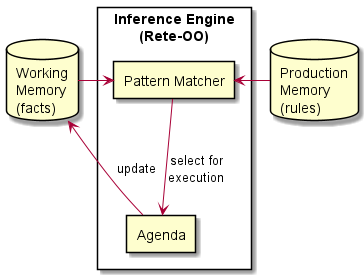
\includegraphics[width=0.55\textwidth]{Sections/images/components.png}}
    \caption{Drools components.}
    \label{fig:Drools_components}
\end{figure}

In Forgy's\cite{forgy1989rete} overview of a rete algorithm, the following steps occur.
\begin{enumerate}
    \item Match: Evaluate the LHSs of the productions to determine which are satisfied given the current contents of working memory.
    \item Conflict resolution: Select one production with a satisfied LHS; halt the interpreter if no productions have satisfied LHSs.
    \item Act: Perform the actions in the RHS of the selected production.
    \item Re-evaluate: Go To 1.
\end{enumerate}

Figure \ref{fig:Drools_inference_loop} show more detail of how these components interact within Drools to infer a conclusion.
First, Drools asserts facts in the working memory.
The working memory contains the current state of the facts, which triggers the inference engine.
Using the aforementioned Rete-OO algorithm, the pattern matcher will examine the working memory and a representation of the rules from the production memory to determine which rules are true.
Drools will then put the rules that match on the agenda.
It can be the case that many rules are concurrently true for the same fact assertion.
These rules conflict.
A conflict resolution strategy will decide which rule will fire in which order from the agenda.
The first rule on the agenda will fire.
If the rule modifies, retracts or asserts a fact, then the inference loop begins again.
We have inferred our conclusion if a rule specifies to halt or there are no matching rules left on the agenda.

\begin{figure}[h]
    \centering
    \fbox{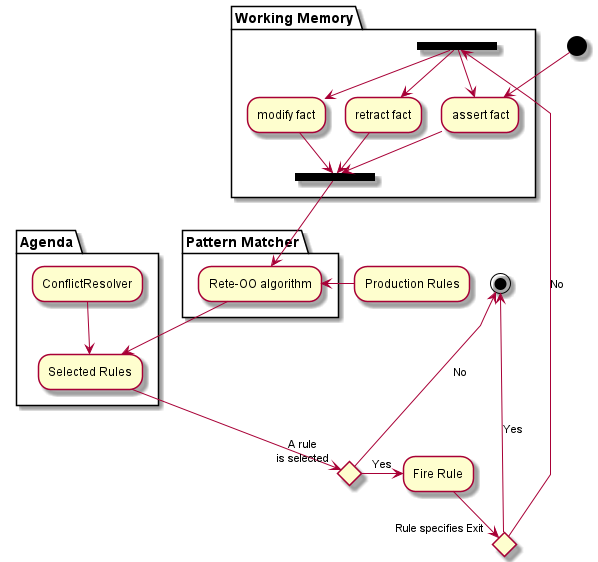
\includegraphics[width=0.55\textwidth]{Sections/images/InferenceLoop-1.png}}
    \caption{Drools inference loop}
    \label{fig:Drools_inference_loop}
\end{figure}

The component we will be focussing on in this paper is the rules.
A rules file containing the rules is a text file, typically with a .drl extension.
As the rules do not change during execution
During execution, the rules do not change, and Drools stores them in production memory.

We do not need to examine the rule file components package, import, global, declare, function and query.
We will examine the anatomy of a rule.

A rule consists of 3 parts: attributes, conditions, and consequences.
Attributes are optional hints to the inference engine as to how to examine a rule.
The conditional, ``when'', or left-hand side (LHS) of the rule statement is a block of conditions that have to, in aggregate, return true for the asserted fact. If true, then the rule is placed on the agenda.
The actions, consequences, ``then'', or right-hand side (RHS) of the rule statement contains actions to be executed when the rule is selected.

The LHS is a predicate statement made up of some patterns.
The patterns evaluate facts from the working memory.
The pattern can match against the existence of facts or facts with matching property conditions.
Connectives, such as not, and, and or can combine patterns.
The patterns apply to individual facts rather than the group, thus can be seen as first-order predicates.

Variables can be bound to facts that match these patterns for use later in the LHS or for updating the working memory on the RHS.

Drools offers more options for the LHS.
We have limited the scope of this paper to the features described thus far.

The RHS can contain arbitrary code that will execute when a rule is selected.
However, its primary purpose is to adjust the state of truth in the working memory.
One can insert, modify, and retract facts in the working memory.
Modifying and retracting facts must be done on fact variable references bound in the LHS.
One can explicitly terminate the inference loop with a halt command.

\begin{figure}[h]
    \centering
    \fbox{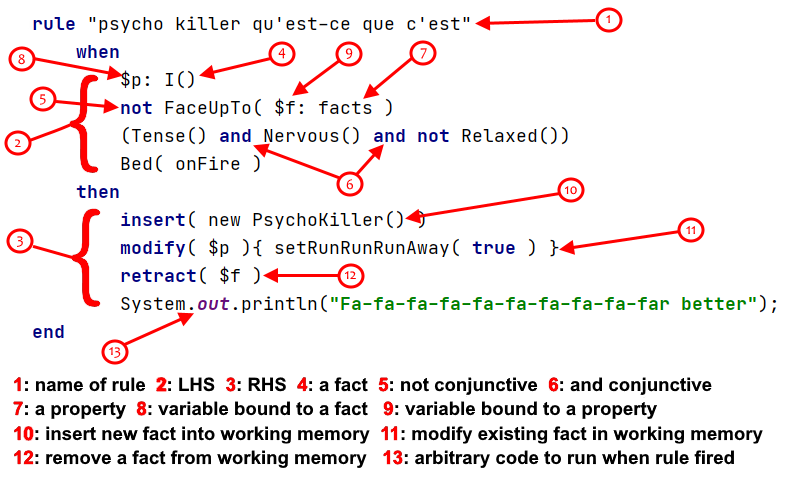
\includegraphics[width=0.95\textwidth]{Sections/images/DroolsRule2.png}}
    \caption{Drools rule breakdown}
    \label{fig:Drools_Rule_Breakdown}
\end{figure}

\subsubsection{An Explanatory Example}
Listing \ref{listing:drl_file} shows an example of a .drl file taken from the Drools sample code.

\noindent\begin{minipage}{\textwidth}
    \begin{lstlisting}[language={[drl]Drools}, caption=Example Drools file., captionpos=b, label=listing:drl_file]
        package org.drools.examples.honestpolitician
    
        import org.drools.examples.honestpolitician.Politician;
        import org.drools.examples.honest politician.Hope;
        
        rule ``We have an honest Politician''
            salience 10
            when
                exists( Politician( honest == true ) )
            then
                insertLogical( new Hope() );
        end
        
        rule ``Hope Lives''
            salience 10
            when
                exists( Hope() )
            then
                System.out.println(``Hurrah!!! Democracy Lives'');
        end
        
        rule ``Hope is Dead''
            when
                not( Hope() )
            then
                System.out.println( ``We are all Doomed!!! Democracy is Dead'' );
        end
        
        rule ``Corrupt the Honest''
            when
                $p : Politician( honest == true )   
                exists( Hope() )
            then
                System.out.println( ``I'm an evil corporation and I have corrupted `` + $p.getName() );
                modify( $p ) { 
                    setHonest( false ) 
                }
        end
    \end{lstlisting}
\end{minipage}

Listing \ref{listing:drl_file} gives the Drools engine instructions on what actions to take when something changes the working memory.
This toy example reacts to when the working memory has an honest politician added. 
It prints a message celebrating the existence of said politician.
It then corrupts her and gloats in a message.
Finally, it prints a message of despair.
The code in Listing \ref{listing:drl_file} does the following: 
\begin{enumerate}[topsep=2pt,itemsep=2pt,partopsep=2pt, parsep=2pt]
    \item On line 1, the package statement identifies the rule file.
    \item On lines 3 and 4, the import statements describe which facts are available for use.
    \item The ``We have an honest Politician'' rule on line 6 does the following:
    \begin{enumerate}[topsep=2pt,itemsep=2pt,partopsep=2pt, parsep=2pt]
        \item On line 7, using the salience attribute, the rule is set to be run before other rules with a lower salience.
        \item On line 10, the rule checks working memory for Politician facts with the honest property equal to true.
        \item On line 12, if found, then a Hope fact is inserted into the working memory.
    \end{enumerate}
    \item The ``Hope Lives'' rule on line 15 does the following:
    \begin{enumerate}[topsep=2pt,itemsep=2pt,partopsep=2pt, parsep=2pt]
        \item Line 18 check if any Hope facts exist.
        \item On line 20, if found, it prints a message.
    \end{enumerate}
    \item The ``Hope is Dead'' rule on line 23 does the following:
    \begin{enumerate}[topsep=2pt,itemsep=2pt,partopsep=2pt, parsep=2pt]
        \item On line 25, it checks that no Hope facts exist.
        \item On line 27, if it finds no facts, then it prints a message.  
    \end{enumerate}
    \item the ``Corrupt the Honest'' rule on line 30 does the following:
    \begin{enumerate}[topsep=2pt,itemsep=2pt,partopsep=2pt, parsep=2pt]
        \item Line 32 checks for any Politician facts with the honest property equal to true and sets them to the variable \$p.
        \item Line 33 checks if any Hope facts exist.
        \item If both Hope and Politician facts are found, on line 35, it prints a message including the \$p variables name.
        \item On lines 36 to 38, it modifies the fact in working memory represented by \$p to change its honest property.
    \end{enumerate}
\end{enumerate}

